\documentclass[conference]{IEEEtran}
\IEEEoverridecommandlockouts

\usepackage{cite}
\usepackage{amsmath,amssymb,amsfonts}
\usepackage{algorithm}
\usepackage{algpseudocode}
\usepackage{graphicx}
\usepackage{textcomp}
\usepackage{xcolor}
\usepackage{booktabs}
\usepackage{multirow}
\usepackage{array}
\usepackage{pifont}
\usepackage{tikz}
\usetikzlibrary{arrows.meta,positioning,fit,calc,shapes.geometric,backgrounds}
\usepackage[hidelinks]{hyperref}

\newcommand{\cmark}{\ding{51}}
\newcommand{\pmark}{$\circ$}
\newcommand{\xmark}{--}
\algrenewcommand\algorithmicrequire{\textbf{Input:}}
\algrenewcommand\algorithmicensure{\textbf{Output:}}

\definecolor{aionnavy}{HTML}{151F49}
\definecolor{aiontint}{HTML}{E4E7F2}
\definecolor{aiongold}{HTML}{B8862F}

\begin{document}

\title{AION: A Closed-Loop, Human-Gated Framework for LLM-Assisted Incident Detection, Root-Cause Analysis, and Validated Remediation}

\author{
\IEEEauthorblockN{Aditya Bheke}
\IEEEauthorblockA{\textit{Dept. of Computer Engineering} \\
\textit{Ajeenkya D Y Patil School of Engineering}\\
Pune, India \\
aditya.bheke@dypic.in}
\and
\IEEEauthorblockN{Harshal Bhogawade}
\IEEEauthorblockA{\textit{Dept. of Computer Engineering} \\
\textit{Ajeenkya D Y Patil School of Engineering}\\
Pune, India \\
harshal.bhogawade@dypic.in}
\and
\IEEEauthorblockN{Malhar Bhoi}
\IEEEauthorblockA{\textit{Dept. of Computer Engineering} \\
\textit{Ajeenkya D Y Patil School of Engineering}\\
Pune, India \\
malhar.bhoi@dypic.in}
\and
\IEEEauthorblockN{Dr. Yogesh Bahendwar}
\IEEEauthorblockA{\textit{Dept. of Computer Engineering} \\
\textit{Ajeenkya D Y Patil School of Engineering}\\
Pune, India}
}

\maketitle

\begin{abstract}
Resolving a production incident still requires engineers to search large volumes of logs, trace the failure to the code change that caused it, write and test a fix, and deploy it under time pressure. Prior work automates individual stages of this process---log parsing and anomaly detection, root-cause analysis (RCA), or automated program repair---but the stages are usually studied in isolation, and repair techniques are evaluated on benchmark bugs disconnected from live telemetry, deployment history and release pipelines. We present AION (Autonomous Incident Observation \& Navigation), a framework that connects these stages in a single closed loop while keeping a human in control of production. AION deduplicates structured logs into error signatures, detects incidents as signature-level error spikes, ranks suspect commits with an explainable weighted score that combines \texttt{git blame}, function scope, dependency overlap and deployment timing, and asks a large language model (LLM) for an evidence-cited diagnosis that is checked against a curated evidence pack. Candidate patches are generated on isolated branches under a code-enforced policy and are accepted only after a deterministic validation pipeline (fail-to-pass regression test, unit tests, staging deployment and replay of the failing requests). Deployment is possible only through an explicit human approval that is bound to the exact validated commit. On four seeded scenarios with known root causes, AION detected every incident with no false positive and ranked the true culprit first in all three faulty releases; with a locally hosted 7B-parameter model, its LLM diagnosis named the culprit in two of three cases, and every incorrect AI patch was rejected by validation before reaching the approval gate.
\end{abstract}

\begin{IEEEkeywords}
AIOps, incident management, log analysis, root-cause analysis, large language models, automated program repair, human-in-the-loop, continuous deployment
\end{IEEEkeywords}

%====================================================================
\section{Introduction}
%====================================================================
Modern software services produce continuous streams of logs, alerts and deployment events. When a release introduces a fault, on-call engineers must find the relevant error among thousands of log lines, decide which recent change caused it, write and test a fix, and push that fix through the deployment pipeline. Empirical studies of cloud incident management report that this process remains expensive and dependent on experienced engineers, even in organisations with mature tooling~\cite{chen2020icm,notaro2021survey}.

Research in AIOps has made substantial progress on each stage separately. Log parsers such as Drain~\cite{he2017drain} and LILAC~\cite{jiang2024lilac} convert raw logs into templates; DeepLog~\cite{du2017deeplog}, LogAnomaly~\cite{meng2019loganomaly}, NeuralLog~\cite{le2021neurallog} and BERT-based detectors~\cite{guo2021logbert,lee2023lanobert,delacruz2026loganomaly} detect anomalous log behaviour. RCA techniques localise faulty services~\cite{wu2020microrca,ma2020automap,soldani2022survey}, and recent work shows that LLMs can recommend root causes and mitigations for real cloud incidents~\cite{ahmed2023recommending,chen2024rcacopilot,roy2024exploring}. In parallel, LLM-based automated program repair (APR) and software engineering agents can generate and test code fixes~\cite{xia2023apr,bouzenia2025repairagent,zhang2024autocoderover,yang2024sweagent}.

Two gaps remain. First, these stages are rarely connected: detection and RCA systems stop at a diagnosis, while repair systems start from a bug report or a failing test and are evaluated on benchmarks such as Defects4J or SWE-bench~\cite{jimenez2024swebench} rather than on live production signals, deployment history and release pipelines. Recent surveys identify this fragmentation, together with hallucination and unreliable evaluation, as open problems for LLM-based AIOps~\cite{zhang2026aiopsllm,ma2026llm4log}. Second, letting an LLM change production code is unsafe without guarantees: a plausible but wrong fix can make an incident worse, and work on LLM-based remediation explicitly calls for safety checks~\cite{integrating2025llmobs}.

AION addresses both gaps with a closed-loop workflow in which AI may \emph{investigate, analyse, propose and validate}, but only a human may \emph{approve} a production change. This paper makes the following contributions:
\begin{itemize}
\item An end-to-end architecture that connects log-based detection, change correlation, LLM diagnosis, patch generation, deterministic validation and deployment, with the human approval gate enforced structurally by a finite-state machine and bound to a commit hash (Section~\ref{sec:arch}).
\item An explainable change-correlation score that combines line- and function-level \texttt{git blame}, file and dependency overlap and deployment timing, extending the classical idea of fix-inducing changes~\cite{sliwerski2005changes} to online incident triage (Section~\ref{sec:corr}).
\item An evidence-pack and grounding scheme that requires every LLM claim to cite a verifiable evidence item and caps confidence when claims cannot be verified (Section~\ref{sec:rca}).
\item A policy-constrained generate--validate--repair loop with fail-to-pass checking, staging request replay and a revert fallback (Sections~\ref{sec:patch}--\ref{sec:valid}).
\item A scenario-based evaluation with known answers that measures each stage separately and documents how the evaluation exposed and fixed four weaknesses of the initial design (Section~\ref{sec:eval}).
\end{itemize}

%====================================================================
\section{Related Work}
%====================================================================
\subsection{Log Parsing and Anomaly Detection}
Surveys of automated log analysis cover the full pipeline from logging practice through parsing, anomaly detection, failure prediction and diagnosis~\cite{he2021survey}, and public datasets such as Loghub~\cite{zhu2023loghub} have enabled systematic benchmarking. Drain~\cite{he2017drain} parses logs online with a fixed-depth tree; LILAC~\cite{jiang2024lilac} uses LLMs with an adaptive parsing cache to improve template accuracy while reducing LLM queries. DeepLog~\cite{du2017deeplog} and LogAnomaly~\cite{meng2019loganomaly} learn normal log sequences; NeuralLog~\cite{le2021neurallog} avoids parsing errors by embedding raw messages; LogBERT~\cite{guo2021logbert} and LAnoBERT~\cite{lee2023lanobert} apply self-supervised BERT models, and a recent industrial deployment runs a LogBERT model locally for confidentiality~\cite{delacruz2026loganomaly}. A systematic review of LLM-based log analysis~\cite{ma2026llm4log} notes log drift, hallucination and context and cost limits. These methods establish \emph{that} something is wrong; they do not identify the responsible change or repair it. AION deliberately uses a lightweight, deterministic detector (template masking plus spike detection), because its contribution lies in what happens after detection.

\subsection{AIOps, Incident Management and Root-Cause Analysis}
Notaro \emph{et al.}~\cite{notaro2021survey} organise AIOps failure-management methods into prevention, detection, diagnosis and remediation, and Zhang \emph{et al.}~\cite{zhang2026aiopsllm} survey how LLMs are changing these tasks. At Microsoft, Chen \emph{et al.}~\cite{chen2020icm} report two years of incident-management practice, and Ahmed \emph{et al.}~\cite{ahmed2023recommending} evaluate GPT-3.x models on more than 40,000 incidents for recommending root causes and mitigation steps from the incident title and summary. LLM-based RCA systems for cloud incidents~\cite{chen2024rcacopilot} and LLM agents for RCA~\cite{roy2024exploring} show that diagnosis improves when the model is given relevant context. Service-level RCA methods such as MicroRCA~\cite{wu2020microrca} and AutoMAP~\cite{ma2020automap} localise faulty microservices from metrics and dependency graphs~\cite{soldani2022survey}, and Wittkopp \emph{et al.}~\cite{wittkopp2023progressing} progress from anomaly detection towards log labelling and RCA. Integrating LLMs with cloud-native observability for automated RCA and remediation~\cite{integrating2025llmobs} highlights the risks of hallucinated root causes and telemetry that exceeds the model's context. AION adopts the lesson that context quality matters, but replaces free-form retrieval with a bounded, citable evidence pack, and it links the diagnosis to a concrete, testable code change.

\subsection{Change Analysis}
The SZZ approach of \'Sliwerski \emph{et al.}~\cite{sliwerski2005changes} links version history to bug reports to identify fix-inducing changes after the fact. AION applies a related intuition online: when an error spike follows a deployment, the commits that touched the failing lines, functions or their dependencies, and that shipped in that deployment, are the strongest suspects.

\subsection{Automated Program Repair and LLM Agents}
Le Goues \emph{et al.}~\cite{legoues2019apr} review search-, semantics- and learning-based APR. AlphaRepair~\cite{xia2022alpharepair} showed that pre-trained code models can repair bugs zero-shot, and Xia \emph{et al.}~\cite{xia2023apr} found that larger pre-trained models outperform earlier APR tools across five datasets; Zhang \emph{et al.}~\cite{zhang2024slr} review the rapidly growing LLM-based APR literature. RepairAgent~\cite{bouzenia2025repairagent} is an autonomous agent that repaired 164 Defects4J bugs; AutoCodeRover~\cite{zhang2024autocoderover} combines program-structure-aware code search with LLMs; SWE-agent~\cite{yang2024sweagent} designs agent--computer interfaces for software engineering; and SWE-bench~\cite{jimenez2024swebench} evaluates such systems on 2,294 real GitHub issues. Kulsum \emph{et al.}~\cite{kulsum2024vrpilot} show that patch-validation feedback improves LLM-generated vulnerability fixes. These systems start from an issue or a failing test and end with a candidate patch; none of them observes production, correlates deployments or gates deployment on human approval.

\subsection{Positioning}
Table~\ref{tab:related} summarises the stages covered by representative work. AION's novelty is not a better individual stage but the safe, auditable composition of all stages, with deterministic checks around every AI output.

\begin{table}[t]
\centering
\caption{Stage coverage of representative work (\cmark{} covered, \pmark{} partial, \xmark{} not covered)}
\label{tab:related}
\setlength{\tabcolsep}{3pt}
\footnotesize
\resizebox{\columnwidth}{!}{%
\begin{tabular}{@{}lcccccc@{}}
\toprule
Work & Det. & Corr. & RCA & Repair & Valid. & Gate \\
\midrule
DeepLog, NeuralLog~\cite{du2017deeplog,le2021neurallog} & \cmark & \xmark & \xmark & \xmark & \xmark & \xmark \\
MicroRCA, AutoMAP~\cite{wu2020microrca,ma2020automap} & \pmark & \xmark & \cmark & \xmark & \xmark & \xmark \\
LLM incident RCA~\cite{ahmed2023recommending,chen2024rcacopilot} & \xmark & \xmark & \cmark & \xmark & \xmark & \xmark \\
SZZ~\cite{sliwerski2005changes} & \xmark & \cmark & \xmark & \xmark & \xmark & \xmark \\
RepairAgent, AutoCodeRover~\cite{bouzenia2025repairagent,zhang2024autocoderover} & \xmark & \xmark & \pmark & \cmark & \cmark & \xmark \\
\textbf{AION (this work)} & \cmark & \cmark & \cmark & \cmark & \cmark & \cmark \\
\bottomrule
\end{tabular}}
\vspace{2pt}

\raggedright\scriptsize Det.: detection from production logs; Corr.: correlation with commits and deployments; Valid.: validation in staging before release; Gate: enforced human approval for production.
\end{table}

%====================================================================
\section{System Architecture}
\label{sec:arch}
%====================================================================
Fig.~\ref{fig:arch} shows the closed loop. A monitored production service emits structured JSON logs. AION, implemented as a modular monolith, processes them through eight stages; stages 1--6 run automatically in a background pipeline, stage 7 requires a human, and stage 8 runs only after approval. Every transition is appended to an audit trail.

\begin{figure*}[t]
\centering
\resizebox{\textwidth}{!}{%
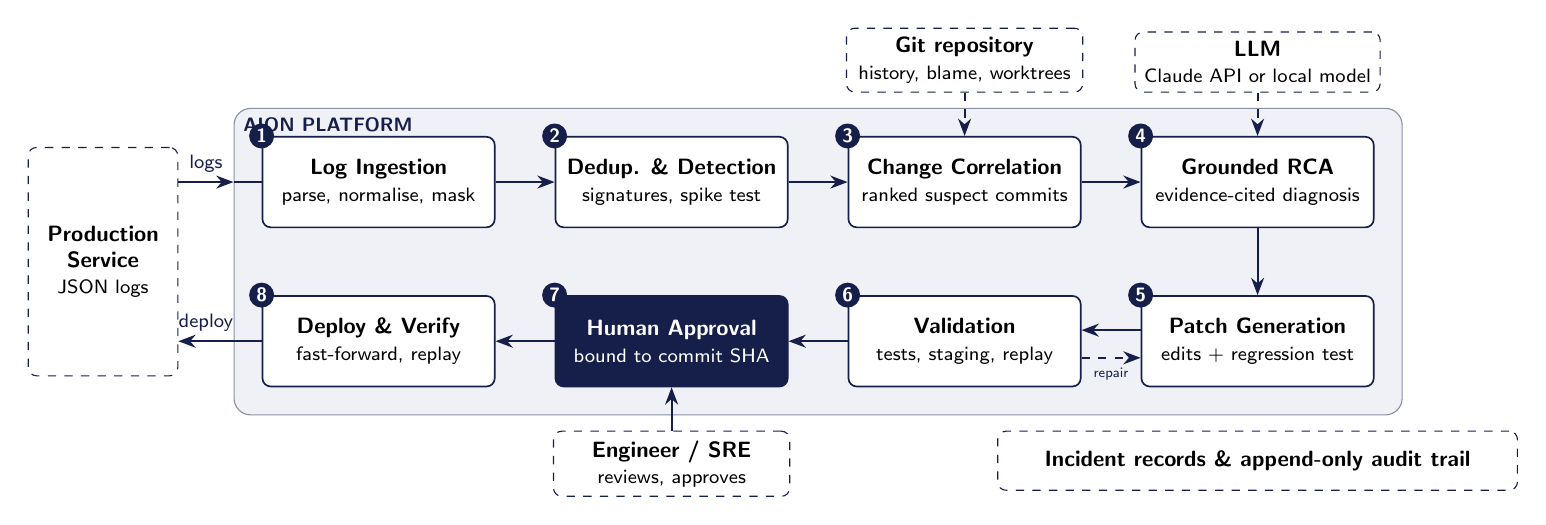
\begin{tikzpicture}[
  font=\sffamily\footnotesize,
  stage/.style={draw=aionnavy, fill=white, rounded corners=3pt, minimum width=2.95cm, minimum height=1.15cm, align=center, line width=0.6pt},
  gate/.style={stage, fill=aionnavy, text=white},
  ext/.style={draw=aionnavy, dashed, rounded corners=3pt, minimum width=3.0cm, minimum height=0.75cm, align=center, fill=white},
  arr/.style={-{Stealth[length=2.2mm]}, line width=0.7pt, color=aionnavy},
  num/.style={circle, fill=aionnavy, text=white, inner sep=1pt, font=\sffamily\scriptsize\bfseries},
]
\node[stage] (s1) at (0,0) {\textbf{Log Ingestion}\\ \scriptsize parse, normalise, mask};
\node[stage, right=0.75cm of s1] (s2) {\textbf{Dedup. \& Detection}\\ \scriptsize signatures, spike test};
\node[stage, right=0.75cm of s2] (s3) {\textbf{Change Correlation}\\ \scriptsize ranked suspect commits};
\node[stage, right=0.75cm of s3] (s4) {\textbf{Grounded RCA}\\ \scriptsize evidence-cited diagnosis};
\node[stage, below=0.85cm of s4] (s5) {\textbf{Patch Generation}\\ \scriptsize edits + regression test};
\node[stage, left=0.75cm of s5] (s6) {\textbf{Validation}\\ \scriptsize tests, staging, replay};
\node[gate, left=0.75cm of s6] (s7) {\textbf{Human Approval}\\ \scriptsize bound to commit SHA};
\node[stage, left=0.75cm of s7] (s8) {\textbf{Deploy \& Verify}\\ \scriptsize fast-forward, replay};
\foreach \n/\k in {s1/1,s2/2,s3/3,s4/4,s5/5,s6/6,s7/7,s8/8}{\node[num] at (\n.north west) {\k};}
\begin{scope}[on background layer]
\node[draw=aionnavy!50, fill=aiontint!60, rounded corners=6pt, fit=(s1)(s4)(s5)(s8), inner sep=0.35cm, label={[font=\sffamily\scriptsize\bfseries, text=aionnavy, anchor=north west]north west:AION PLATFORM}] (plat) {};
\end{scope}
\node[ext, anchor=east, minimum height=2.9cm, minimum width=1.9cm] (prod) at ($(plat.west)+(-0.7,0)$) {\textbf{Production}\\\textbf{Service}\\ \scriptsize JSON logs};
\node[ext, above=0.55cm of s3] (git) {\textbf{Git repository}\\ \scriptsize history, blame, worktrees};
\node[ext, above=0.55cm of s4] (llm) {\textbf{LLM}\\ \scriptsize Claude API or local model};
\node[ext, below=0.55cm of s7] (eng) {\textbf{Engineer / SRE}\\ \scriptsize reviews, approves};
\node[ext, below=0.55cm of s5, minimum width=6.6cm] (aud) {\textbf{Incident records \& append-only audit trail}};
\draw[arr] (s1) -- (s2); \draw[arr] (s2) -- (s3); \draw[arr] (s3) -- (s4); \draw[arr] (s4) -- (s5);
\draw[arr] ([yshift=4pt]s5.west) -- ([yshift=4pt]s6.east); \draw[arr] (s6) -- (s7); \draw[arr] (s7) -- (s8);
\draw[arr, dashed] ([yshift=-6pt]s6.east) -- node[below, font=\sffamily\tiny]{repair} ([yshift=-6pt]s5.west);
\draw[arr] (prod.east |- s1) -- node[above, font=\sffamily\scriptsize]{logs} (plat.west |- s1);
\draw[arr] (plat.west |- s8) -- node[above, font=\sffamily\scriptsize]{deploy} (prod.east |- s8);
\draw[color=aionnavy, line width=0.7pt] (s1.west) -- (plat.west |- s1); \draw[color=aionnavy, line width=0.7pt] (s8.west) -- (plat.west |- s8);
\draw[arr, dashed] (git) -- (s3); \draw[arr, dashed] (llm) -- (s4);
\draw[arr] (eng) -- (s7);
\end{tikzpicture}}
\caption{AION closed-loop architecture. Stages 1--6 run automatically; production deployment (stage 8) is reachable only through an explicit human approval (stage 7). Failed validation loops back to patch generation a bounded number of times.}
\label{fig:arch}
\end{figure*}

\subsection{Design Principles}
\begin{itemize}
\item \textbf{AI proposes, humans dispose.} The incident lifecycle is a finite-state machine (Fig.~\ref{fig:fsm}); no transition leads from \textsc{awaiting\_approval} to \textsc{deploying} except through \textsc{approved}, which only the human approval API can enter.
\item \textbf{Deterministic checks around every AI output.} LLM diagnoses are grounded against evidence; LLM patches pass a code-enforced policy and a validation pipeline whose commands are defined by the operator, never by the model.
\item \textbf{Explainability.} Every suspect score, grounding warning and validation step is stored with a human-readable reason.
\item \textbf{Graceful degradation.} Without an LLM, a clearly labelled deterministic analyser reports the top-ranked suspect and proposes a \texttt{git revert}.
\end{itemize}

\begin{figure}[t]
\centering
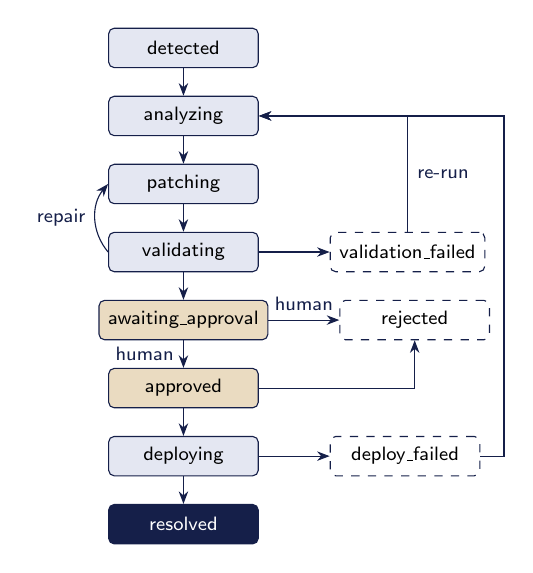
\begin{tikzpicture}[
  font=\sffamily\scriptsize,
  st/.style={draw=aionnavy, rounded corners=2pt, fill=aiontint, minimum width=1.9cm, minimum height=0.5cm, align=center},
  bad/.style={st, fill=white, dashed},
  hum/.style={st, fill=aiongold!30},
  arr/.style={-{Stealth[length=1.6mm]}, color=aionnavy},
]
\node[st] (det) at (0,0) {detected};
\node[st, below=0.35cm of det] (ana) {analyzing};
\node[st, below=0.35cm of ana] (pat) {patching};
\node[st, below=0.35cm of pat] (val) {validating};
\node[hum, below=0.35cm of val] (wait) {awaiting\_approval};
\node[hum, below=0.35cm of wait] (app) {approved};
\node[st, below=0.35cm of app] (dep) {deploying};
\node[st, below=0.35cm of dep, fill=aionnavy, text=white] (res) {resolved};
\node[bad, right=0.9cm of val] (vf) {validation\_failed};
\node[bad, right=0.9cm of wait] (rej) {rejected};
\node[bad, right=0.9cm of dep] (df) {deploy\_failed};
\draw[arr] (det)--(ana); \draw[arr] (ana)--(pat); \draw[arr] (pat)--(val); \draw[arr] (val)--(wait);
\draw[arr] (wait)--node[left]{human}(app); \draw[arr] (app)--(dep); \draw[arr] (dep)--(res);
\draw[arr] (val)--(vf); \draw[arr] (wait)--node[above]{human}(rej); \draw[arr] (dep)--(df);
\draw[arr] (val.west) to[bend left=40] node[left]{repair} (pat.west);
\draw[arr] (vf.north) |- node[pos=0.25, right]{re-run} (ana.east);
\draw[arr] (df.east) -- ++(0.3,0) |- (ana.east);
\draw[arr] (app.east) -| (rej.south);
\end{tikzpicture}
\caption{Incident lifecycle. Shaded states require a human decision; there is no automated edge into \textsc{approved}.}
\label{fig:fsm}
\end{figure}

%====================================================================
\section{Methodology}
%====================================================================
\subsection{Log Normalisation and Signatures}
Each log record $l$ is normalised into an event with timestamp, level, message, request context and parsed stack frames. A template $\tau(l)$ is obtained by masking variable fields in a fixed order---UUIDs, URLs, e-mail and IP addresses, hexadecimal identifiers, timestamps and finally numbers---so that \emph{``Order 1042 failed after 3.2ms''} becomes \emph{``Order \textless NUM\textgreater{} failed after \textless NUM\textgreater ms''}. For error events, the signature is a hash
\begin{equation}
s(l) = h\big(\text{type}(l),\ \text{frames}(l),\ \tau(l)\big),
\end{equation}
where $\text{frames}(l)$ are the innermost application frames (file and function, deliberately \emph{without} line numbers so that a signature survives unrelated edits). Signatures are stored with occurrence counts and first and last occurrence times.

\subsection{Incident Detection}
Let $c_t(s)$ be the number of events with signature $s$ in the current window of length $W$, and $b(s)$ the average number of occurrences per window over the preceding baseline period $B$. An incident is opened when
\begin{equation}
c_t(s) \ge m \quad\wedge\quad c_t(s) \ge \rho \cdot b(s),
\label{eq:spike}
\end{equation}
with defaults $W=60$\,s, $B=30$\,min, $m=5$ and $\rho=3$. A brand-new error ($b(s)=0$) fires once it reaches $m$, while long-standing low-rate noise does not. Further events with the same signature attach to the open incident, and event time (not wall-clock time) is used, so replayed logs behave identically to live traffic. Events older than the closure of a previous incident with the same signature are ignored, preventing late log lines from reopening a fixed problem.

\subsection{Change Correlation}
\label{sec:corr}
For each commit $c$ in the recent history of the service, AION computes binary or graded signals $f_k(c)$ and combines them into an explainable suspicion score
\begin{equation}
S(c) = \min\Big(1,\ \sum_k w_k\, f_k(c)\Big)\cdot \lambda(c),
\qquad c^\ast = \arg\max_c S(c),
\label{eq:score}
\end{equation}
with the signals and weights of Table~\ref{tab:weights}. Blame signals are computed at the \emph{deployed} revision, function ranges are found with Python's \texttt{ast} module, and signals from deeper stack frames are damped by 0.5. Each signal counts once per commit, so a commit touching many frames cannot inflate its score. Commits already running in an earlier deployment before the errors appeared receive $\lambda(c)=0.5$; otherwise $\lambda(c)=1$. Ties are broken by recency. $S(c)$ is a ranking heuristic, not a probability; the LLM later reasons over the top candidates and their diffs.

\begin{table}[t]
\centering
\caption{Change-correlation signals and weights}
\label{tab:weights}
\footnotesize
\begin{tabular}{@{}p{2.3cm}p{4.6cm}c@{}}
\toprule
Signal & Condition & $w_k$ \\
\midrule
Blame (line) & commit last modified the failing line & 0.40 \\
Blame (function) & commit modified the enclosing function & 0.20 \\
Deployment timing & commit shipped in the deployment preceding the errors & 0.20 \\
File overlap & commit touched a file in the stack trace & 0.15 \\
Dependency overlap & commit touched a module imported by a file in the trace & 0.15 \\
Keywords & error identifiers appear in the commit message & 0.05 \\
\bottomrule
\end{tabular}
\end{table}

\subsection{Evidence Pack and Grounded Root-Cause Analysis}
\label{sec:rca}
Instead of placing raw logs in the prompt or retrieving free text~\cite{lewis2020rag}, AION assembles a bounded \emph{evidence pack} $E$ whose items carry stable identifiers: deduplicated log clusters (\texttt{LOG-n}, classified as incident, new or pre-existing noise), a representative trace with failing requests (\texttt{TRACE-1}), preceding deployments (\texttt{DEPLOY-n}), top suspects with scores, reasons and diffs (\texttt{COMMIT-x}), the source of the functions in the trace at the deployed revision (\texttt{CODE-n}), and similar past incidents with their fixes (\texttt{INC-n}). The LLM must return structured JSON that separates \emph{observations} (each citing an evidence ID) from \emph{inferences} (each citing supporting evidence), together with affected files, a suspected commit, a remediation plan and a confidence value.

A grounding step then checks the response deterministically: observations citing unknown IDs are removed; inferences without valid support are flagged; affected files must exist in the repository; and the suspected commit must be one of the candidates. Any unverifiable claim caps the confidence at 0.60, and a diagnosis with no verifiable observation is capped at 0.30. The exact evidence pack is stored with the report, so a reviewer sees what the model saw. The provider layer is model-neutral: AION supports the Claude API with structured outputs and any OpenAI-compatible endpoint, including locally hosted models, which keeps sensitive logs on premises.

\subsection{Policy-Constrained Patch Generation}
\label{sec:patch}
Each patch attempt runs in its own Git worktree and branch. The LLM returns search/replace edits plus a regression test that should reproduce the incident; edits whose search text differs from the source only in indentation are repaired automatically. A code-enforced policy, independent of the prompt, rejects patches that edit tests, CI or dependency files, touch non-existent or unsafe paths, change more than five files or more than 200 lines, or place new tests outside a dedicated name pattern. Algorithm~\ref{alg:repair} shows the bounded generate--validate--repair loop: validation failures are fed back to the model for a limited number of attempts, after which AION falls back to reverting the top-ranked suspect commit. Both kinds of candidate go through the same validation and the same human gate.

\begin{algorithm}[t]
\caption{Generate--validate--repair with revert fallback}
\label{alg:repair}
\small
\begin{algorithmic}[1]
\Require incident $I$, evidence pack $E$, diagnosis $R$, suspects $C$, attempt budget $N$
\Ensure validated candidate $P$, or escalation to an engineer
\State $fb \gets \emptyset$
\For{$i = 1$ \textbf{to} $N$}
  \State $P \gets \textsc{LLMPatch}(E, R, fb)$ \Comment{edits + regression test}
  \State $P \gets \textsc{RepairIndentation}(P)$
  \If{$\neg\,\textsc{Policy}(P)$} $fb \gets$ violation; \textbf{continue} \EndIf
  \State $V \gets \textsc{Validate}(P)$ \Comment{Sec.~\ref{sec:valid}}
  \If{$V.\text{passed}$} \Return $P$ \Comment{to approval gate} \EndIf
  \State $fb \gets V.\text{failures}$
\EndFor
\State $P \gets \textsc{Revert}(\arg\max_{c \in C} S(c))$
\If{$\textsc{Validate}(P).\text{passed}$} \Return $P$ \EndIf
\State \Return \textsc{Escalate}$(I)$ \Comment{state \textsc{validation\_failed}}
\end{algorithmic}
\end{algorithm}

\subsection{Deterministic Validation}
\label{sec:valid}
A patch $P$ is accepted only if
\begin{multline}
V(P) = \text{syntax} \wedge \text{fail2pass} \wedge \text{tests} \\
\wedge\ \text{staging} \wedge \text{replay},
\end{multline}
where \emph{syntax} compiles every changed file; \emph{fail2pass} runs the new regression test against the \emph{unpatched} code (where it must fail, proving it reproduces the incident) and against the patch; \emph{tests} runs the service's full test suite; \emph{staging} starts the patched service from its worktree and waits for its health check; and \emph{replay} re-sends the production requests that failed during the incident (expecting no 5xx response) together with a sample of previously successful requests (expecting unchanged status). All commands come from the operator's service registration and run without a shell and with timeouts. This mirrors the finding that validation feedback is essential for trustworthy LLM fixes~\cite{kulsum2024vrpilot}, but executes it against reproduced production traffic rather than a benchmark test suite.

\subsection{Human Approval, Deployment and Audit}
An engineer reviews the evidence, diagnosis, diff and validation report in a web dashboard and approves or rejects the candidate. The approval records the approver, a comment and the commit SHA; deployment is a separate action that re-checks that the approved SHA equals the validated SHA:
\begin{multline}
\text{deploy}(P) \iff V(P)=1 \ \wedge\ A=\text{approve} \\
\wedge\ \text{sha}(A)=\text{sha}(P).
\end{multline}
Deployment is a GitOps-style fast-forward of the production branch, followed by verification that the service reports the approved commit and that the previously failing requests now succeed. The incident is marked resolved only after verification; a failed verification returns it for re-investigation. All actions by the pipeline and by humans are written to an append-only audit table.

%====================================================================
\section{Implementation}
%====================================================================
AION is implemented in Python with FastAPI, SQLAlchemy and SQLite (write-ahead logging) for persistence, the Git command-line tool for history, blame, worktrees and reverts, and a React dashboard that shows a live pipeline view, evidence, diffs, the approval panel and the audit log. A single background worker executes the pipeline. The LLM layer supports the Claude API through the official SDK and OpenAI-compatible servers such as Ollama. A realistic demonstration service---an orders API with a synthetic multi-commit, multi-deployment Git history---is monitored end to end. The code base is covered by 44 automated tests, including complete end-to-end workflow tests. In a live demonstration on a laptop, an injected fault reached the approval gate about 4\,s after the first errors with the deterministic analyser, and approval plus deployment reached a verified, resolved state in about 2\,s.

%====================================================================
\section{Evaluation}
\label{sec:eval}
%====================================================================
\subsection{Research Questions}
\textbf{RQ1:} Does AION detect seeded incidents without false positives? \textbf{RQ2:} Does change correlation rank the true culprit first? \textbf{RQ3:} Does the LLM diagnosis identify the culprit, and do AI patches pass validation? \textbf{RQ4:} Does the safety design stop incorrect patches before the approval gate?

\subsection{Setup}
We built four scenarios on the same five-commit base history of the demonstration service, each with a known answer (Table~\ref{tab:scen}). The \emph{supplier-feed} scenario is deliberately hard: the culprit commit changes only \emph{data}, so \texttt{git blame} on the failing line points at older, innocent code. For each scenario an evaluation harness creates a fresh workspace and database, builds the Git history, executes the real service code to generate normal traffic and trigger requests, ingests the resulting logs through the API and runs the real pipeline up to the approval gate; production deployment is excluded because it always requires a human. We compare two modes: \emph{heuristic} (no LLM: correlation-ranked diagnosis and revert) and \emph{LLM}, using qwen2.5-coder:7b (Q4\_K\_M quantisation) served locally by Ollama on a laptop GPU with 6\,GB of memory, a 12k-token context and temperature 0.1, with at most two AI patch attempts.

\begin{table}[t]
\centering
\caption{Evaluation scenarios (known answers)}
\label{tab:scen}
\footnotesize
\begin{tabular}{@{}p{1.75cm}p{2.25cm}p{3.75cm}@{}}
\toprule
Scenario & Fault & What it tests \\
\midrule
expired-coupon & \texttt{TypeError} on expired coupon & culprit changed the crashing line \\
supplier-feed & \texttt{KeyError: 'price'} & culprit changed only data; blame points at old code \\
empty-cart-average & \texttt{ZeroDivision}\-\texttt{Error} & latent condition becomes fatal after a new feature \\
healthy-release & none & false-positive check with background noise \\
\bottomrule
\end{tabular}
\end{table}

\subsection{Results}
Table~\ref{tab:results} reports the final results. \textbf{RQ1:} both modes detected all three incidents and correctly stayed silent on the healthy release. \textbf{RQ2:} the true culprit was ranked first in all three faulty scenarios, including supplier-feed, where it was found through the dependency-overlap signal (the top two scores tied at 0.40 and the tie was broken by recency). \textbf{RQ3:} the local LLM explained all three failures in plain language and named the culprit commit in two of three cases (confidence 0.9); in supplier-feed it described the symptom but named no commit. None of the six AI-generated patches passed validation. \textbf{RQ4:} every incorrect AI patch was rejected by deterministic checks, and the revert fallback produced validated candidates for two of the three incidents; the third was escalated as \textsc{validation\_failed}. No incorrect patch reached the approval gate in any run.

\begin{table}[t]
\centering
\caption{Final evaluation results}
\label{tab:results}
\footnotesize
\setlength{\tabcolsep}{4pt}
\begin{tabular}{@{}lcc@{}}
\toprule
Metric & Heuristic & Local LLM (7B) \\
\midrule
Detection correct (incl.\ no false positive) & 4/4 & 4/4 \\
True culprit ranked first by correlation & 3/3 & 3/3 \\
Diagnosis names true culprit & 3/3 & 2/3 \\
AI patches passing validation & -- & 0/6 \\
Reached approval gate or correctly silent & 4/4 & 3/4 \\
Incorrect patches reaching the gate & 0 & 0 \\
Mean time per incident & $\approx$5\,s & $\approx$100\,s \\
Mean LLM tokens in / out per incident & -- & $\approx$13.5k / 1.2k \\
\bottomrule
\end{tabular}
\end{table}

\subsection{Evaluation-Driven Improvements}
The evaluation was run five times while the system was improved, and each run exposed a concrete weakness (Table~\ref{tab:runs}). In the first run, \texttt{git blame} ranked the supplier-feed culprit third and every LLM patch failed the syntax check because of indentation errors. Adding the dependency-overlap signal and restricting the keyword signal to the specific error moved the culprit to rank one in all scenarios; indentation-only repair made AI patches compile and produced regression tests that correctly failed on the buggy code, although the fixes themselves remained semantically wrong. A third AI attempt did not help the 7B model, whereas a revert fallback rescued two incidents. All changes were generic and covered by unit tests, rather than tuned to individual scenarios.

\begin{table}[t]
\centering
\caption{Evaluation-driven improvements (gate = reached approval gate or correctly silent; RCA = diagnosis names culprit)}
\label{tab:runs}
\footnotesize
\setlength{\tabcolsep}{3pt}
\resizebox{\columnwidth}{!}{%
\begin{tabular}{@{}clcc@{}}
\toprule
Run & Change since previous run & Heur.\ gate/RCA & LLM gate/RCA \\
\midrule
1 & initial design & 3/4 \,·\, 2/3 & 1/4 \,·\, 2/3 \\
2 & dependency signal, scoped keywords & 4/4 \,·\, 3/3 & -- \\
3 & indentation-only edit repair & -- & 1/4 \,·\, 2/3 \\
4 & three AI attempts instead of two & -- & 1/4 \,·\, 2/3 \\
5 & revert fallback after failed AI patches & 4/4 \,·\, 3/3 & 3/4 \,·\, 2/3 \\
\bottomrule
\end{tabular}}
\end{table}

\subsection{Failure Analysis of AI Patches}
Table~\ref{tab:fail} lists why the local model's patches failed. In empty-cart-average the fix itself was correct, but the model's regression test exercised the wrong order; in expired-coupon the guard was incomplete; in supplier-feed the model ``fixed'' the crash by silently pricing the product at zero. Each failure was caught by a different deterministic check, which supports the design decision to treat every AI output as untrusted until validated.

\begin{table}[t]
\centering
\caption{Why the 7B model's patches failed}
\label{tab:fail}
\footnotesize
\begin{tabular}{@{}p{1.9cm}p{3.9cm}p{2.0cm}@{}}
\toprule
Scenario & Model behaviour & Caught by \\
\midrule
empty-cart-average & correct fix, but regression test used a non-empty order & its own regression test \\
expired-coupon & guarded one field of \texttt{None}, still read another & its own regression test \\
supplier-feed & priced the product at 0 instead of reading the new field & existing unit tests \\
\bottomrule
\end{tabular}
\end{table}

%====================================================================
\section{Discussion}
%====================================================================
\textbf{Diagnosis versus repair.} With a small local model, diagnosis was considerably more reliable than repair: the model explained every failure but produced no validated fix. This matches observations that repair quality grows with model size~\cite{xia2023apr} and that agents need validation feedback~\cite{kulsum2024vrpilot,bouzenia2025repairagent}. Because AION's provider layer is model-neutral, the same harness can measure stronger hosted models with a configuration change.

\textbf{Safety by construction.} The approval guarantee does not depend on model behaviour: it is a property of the state machine, the SHA binding and the operator-defined validation commands. The evaluation shows the value of this separation: every wrong patch was stopped automatically, and every remaining decision went to a human.

\textbf{Explainable correlation.} The weighted score is simple, but every component is a human-readable reason, which helps reviewers and also guides the LLM. The supplier-feed case shows that blame alone is insufficient when the culprit changes data rather than code; the dependency-overlap signal addressed this generically.

\subsection{Limitations and Threats to Validity}
The evaluation is small (four self-authored scenarios on one Python service) and each configuration was run once, so LLM variance is not measured; the results characterise behaviour and failure modes rather than general accuracy. Prompt guidance was adjusted after observing failures; to limit overfitting, every change was generic and unit-tested. Detection uses logs only, with fixed thresholds and hand-tuned weights. Staging and production are local processes, request replay covers idempotent requests only, and AI-generated code is validated in a separate process rather than a container sandbox. The current version has no authentication or role-based approvers, and logs may contain sensitive data when an external LLM is used; a local-model option mitigates the latter.

%====================================================================
\section{Conclusion and Future Work}
%====================================================================
AION shows that log-based detection, change correlation, LLM diagnosis, patch generation, validation and deployment can be connected in a single closed loop without giving AI the authority to change production. In our evaluation, detection and correlation were accurate and deterministic, a 7B local model was useful for diagnosis but not for repair, and deterministic validation together with a commit-bound human gate stopped every incorrect patch. Future work includes evaluating stronger hosted models with repeated runs, a larger benchmark of seeded incidents, metrics- and trace-based detection, support for further languages, integration with real CI/CD systems and container-based staging, sandboxed validation, secret redaction before prompting, role-based approval, and automatic rollback on failed verification.

\bibliographystyle{IEEEtran}
\bibliography{references}

\end{document}
